\setcounter{section}{3} % This causes the next section to be Appendix B


\section*{Examples III. Linear Viscoelastic Models}
\label{PS3}
\medskip
\subsection*{3--1. \textbf{Converting creep to relaxation} [4 pts].} 
First, for part a, the creep time is a sum of the terms:
\begin{equation}
    \tau_c = \frac{8}{3}
\end{equation}
which is marked on the following plot:
\begin{figure}[H]
    \centering
    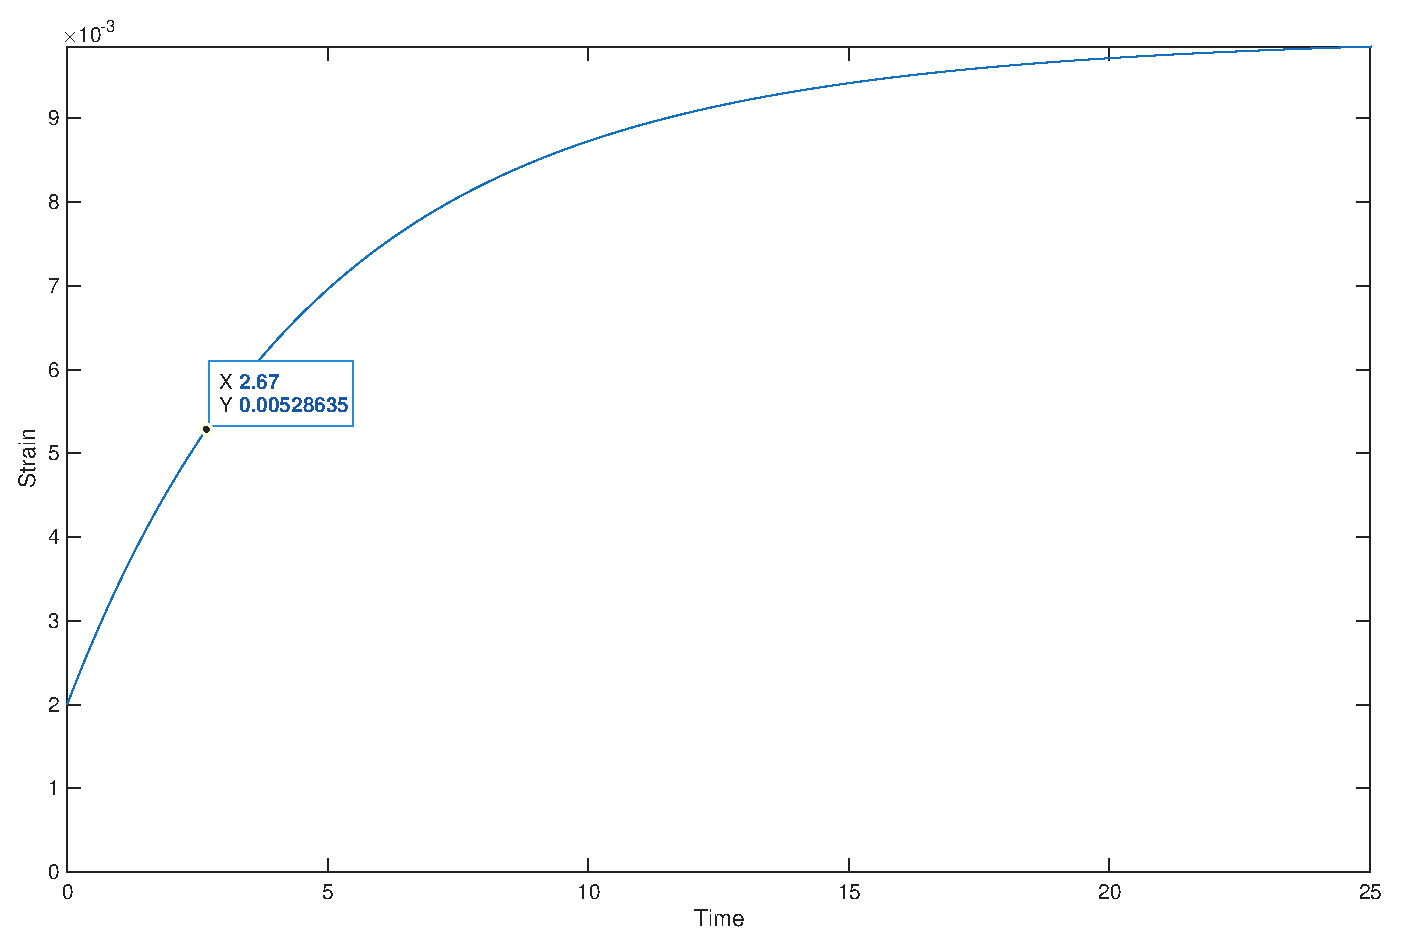
\includegraphics[width=0.7\linewidth]{hw-figures/HW3_P1a.eps}
    \caption{Strain vs Time plot}
    \label{fig:P1a}
\end{figure}
now for the corresponding stress relaxation time
\begin{equation}
    G_r = \mathcal{L}^{-1}(s^2*\mathcal{L}(J_c))
\end{equation}
\begin{equation}
     G_r(t) = \frac{100}{67} \left(-9 \sqrt{201} e^{\left(\frac{\sqrt{201}}{32}-\frac{19}{32}\right) t}+9 \sqrt{201} e^{\left(-\frac{\sqrt{201}}{32}-\frac{19}{32}\right) t}+134 e^{\left(\frac{\sqrt{201}}{32}-\frac{19}{32}\right) t}+134 e^{\left(-\frac{\sqrt{201}}{32}-\frac{19}{32}\right) t}+67\right)
\end{equation}
which has a relaxation time of:
\begin{equation}
    \tau = \frac{1}{\frac{\sqrt{201}}{8}-\frac{19}{8}} = ~1.65
\end{equation}
\begin{figure}[H]
    \centering
    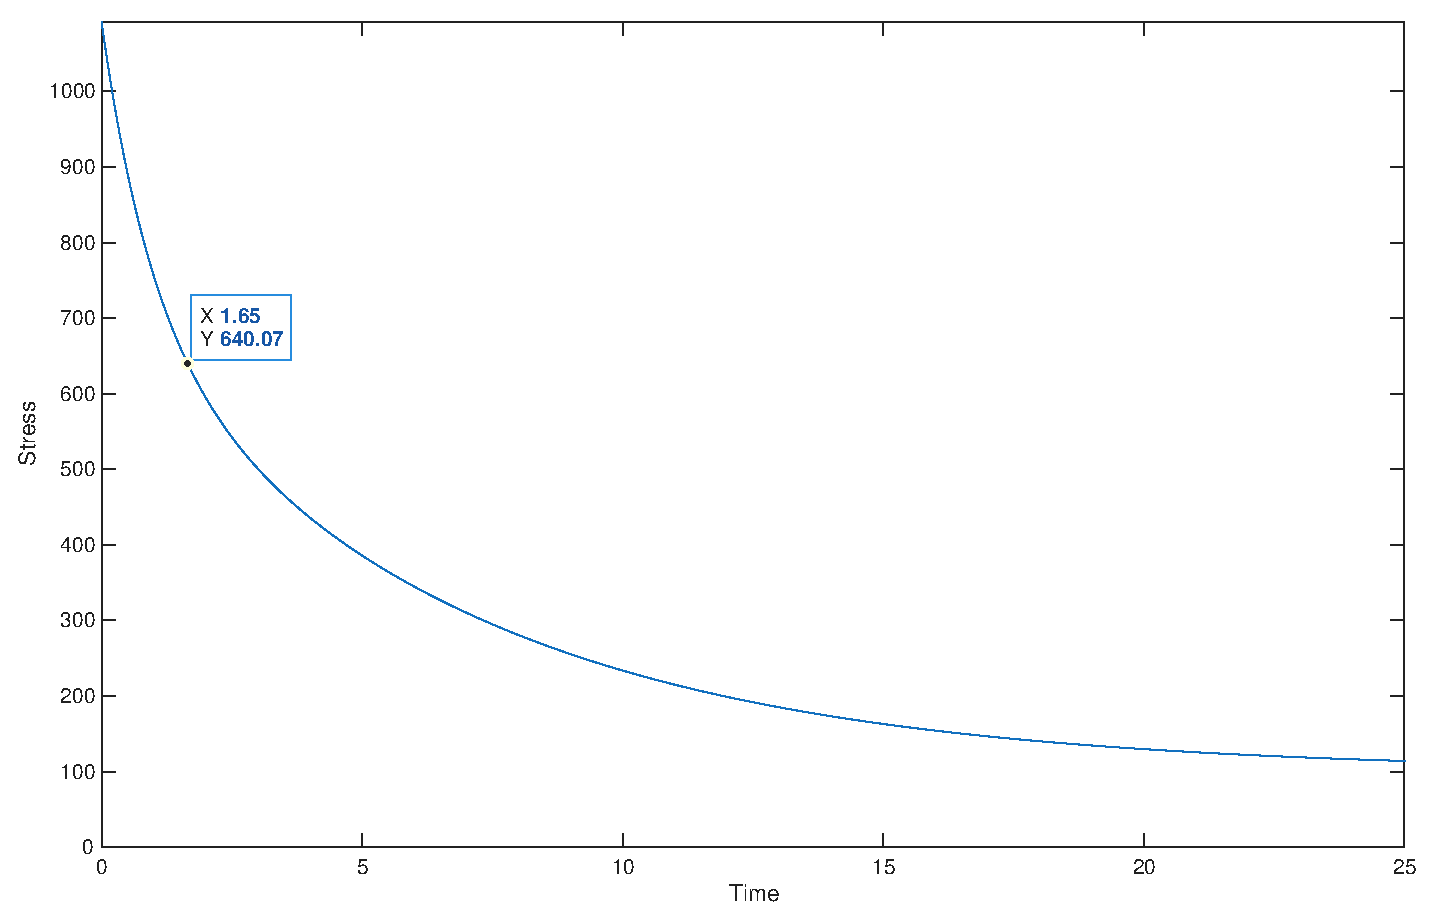
\includegraphics[width=0.7\linewidth]{hw-figures/HW3_P1b.eps}
    \caption{Stress vs Time plot}
    \label{fig:P1b}
\end{figure}
and as we can see from our calculations, the relaxation time is less than the creep time, which is expected!

\bigskip
\bigskip
\bigskip
\subsection*{3--2. \textbf{Alternate standard linear solid model} [4 pts].}
First, defining the series spring (S1) as $E_1$, the KV spring(S2) as $E_2$ and the KV dashpot(D) as $\eta$, we can build our guiding relations:
\begin{equation}
    \sigma = \sigma_{S1}=\varepsilon_{KV}
\end{equation}
\begin{equation}
    \varepsilon = \varepsilon_{S1}+ \varepsilon_{KV}
\end{equation}

First lets convert our stress equation:
\begin{equation}
    \sigma = \eta \dot{\varepsilon}_{KV}+ E_2 \varepsilon_{KV}
\end{equation}
then rearranging:
\begin{equation}
    \varepsilon_{KV} = \varepsilon-\varepsilon_{S1}
\end{equation}
turning that into:
\begin{equation}
    \varepsilon_{KV}= \varepsilon-\frac{\sigma}{E_1}
\end{equation}
and time derivative:
\begin{equation}
    \dot{\varepsilon}_{KV}= \dot{\varepsilon}-\frac{\dot{\sigma}}{E_1}
\end{equation}
plugging in:
\begin{equation}
    \sigma = \eta (\dot{\varepsilon}-\frac{\dot{\sigma}}{E_1})+ E_2(\varepsilon-\frac{\sigma}{E_1})
\end{equation}
rearranging a bit:
\begin{equation}
    \boxed{(E_1+E_2)\sigma+\eta\dot{\sigma}=\eta E_1\dot{\varepsilon}+E_1E_2\varepsilon}
\end{equation}
now, for creep compliance function we take laplace:
\begin{equation}
    \overline{\sigma}(s)(E_1+E_2+\eta s) = \overline{\varepsilon}(\eta E_1 s + E_1E_2)
\end{equation}
then rearranging:
\begin{equation}
    \overline{\sigma}(s) = \frac{\eta E_1 s + E_1E_2}{E_1+E_2+\eta s}\overline{\varepsilon}
\end{equation}
and into Gr
\begin{equation}
    s*\overline{G}_r(s) =\frac{\eta E_1 s + E_1E_2}{E_1s+E_2s+\eta s^2}
\end{equation}
and taking inverse laplace:
\begin{equation}
    \boxed{G_r(t) = \frac{E_1\left(e^{-\frac{E_1+E_2}{\eta}t}\right)E_1+E_2}{E_1+E_2}}
\end{equation}
then transmuting Gr into Jc
\begin{equation}
    \boxed{J_c(t) = \frac{E_1-e^{-\frac{E_2}{\eta}t}E_1+E_2}{E_1E_2}}
\end{equation}
From this we see that the coefficients appear to be very similar in their relations, but opposite with regards to Gr and Jc, where now Jc has the simpler relation and Gr having the more complex versus the Spring in parallel with maxwell. This makes sense considering how solving in certain directions is easier, and in this case solving for Jc would be easier, while the spring parallel with maxwell solving for Gr is. 



\bigskip
\bigskip
\bigskip
\subsection*{3--3. \textbf{Frequency response of a 5-term analog model} [4 pts].}

First, I draw the analog model here:
\begin{figure}[H]
    \centering
    \includegraphics[width=0.3\linewidth]{hw-figures/HW3_P3a.PNG}
    \caption{Diagram of mechanical analog model}
    \label{fig:P3a}
\end{figure}


Then, starting with the given parameter fit, to find the storage and loss moduli we must break it up into the transient and non transient part:
\begin{equation}
    G_r(t) = E_{\infty}+\tilde{E}(t)
\end{equation}
where
\begin{equation}
   E_{\infty} =  G_r(\infty) = C_r (200 e^{-\infty} + 100 e^{-\infty} + 10) = 10 C_r
\end{equation}
this leaves us with:
\begin{equation}
   \tilde{E}(t) =  C_r (200 e^{-\infty} + 100 e^{-\infty})
\end{equation}
following the use of a shifted sinusoid for the strain:
\begin{equation}
    \varepsilon(t) = \varepsilon_0 e^{i\omega t}
\end{equation}
we plug this into our stress eqn:
\begin{equation}
    \sigma(t) = \int_{-\infty}^t G_r(t-\tau) \frac{d\varepsilon}{d\tau}d\tau
\end{equation}
but since we broke up the relaxation function, we get two portions:
\begin{equation}
    \sigma(t) = 10C_r\varepsilon_0 e^{i\omega t}+\int_{-\infty}^tC_r (200 e^{-2t+2\tau} + 100 e^{-t+\tau})i\omega \varepsilon_0 e^{i\omega \tau}d\tau
\end{equation}
following the change of variable: $t' = t-\tau$ 
\begin{equation}
    \sigma(t) = 10 C_r\varepsilon e^{i\omega t}+i\omega \varepsilon_0\int_{0}^{\infty}C_r (200 e^{-2t'} + 100 e^{-t'}) e^{i\omega t}e^{-i\omega t'}dt'
\end{equation}
pulling out variables and expanding:
\begin{equation}
    \sigma(t) =\varepsilon_0 e^{i\omega t}\left[ C_r 10  + i\omega \int_{0}^{\infty}C_r(200 e^{-2t'} + 100 e^{-t'})\cos(\omega t')dt'+\omega\int_{0}^{\infty}C_r(200 e^{-2t'} + 100 e^{-t'})\sin(\omega t')dt'\right]
\end{equation}
now fitting this into the final form:
\begin{equation}
    \sigma(t) = E^*(\omega)\varepsilon(t) =  (E'+iE'')\varepsilon(t)
\end{equation}
with
\begin{equation}
    E'(\omega) = C_r 10 +\omega\int_{0}^{\infty}C_r(200 e^{-2t'} + 100 e^{-t'})\sin(\omega t')dt'
\end{equation}
and
\begin{equation}
    E''(\omega)  =\omega \int_{0}^{\infty}C_r(200 e^{-2t'} + 100 e^{-t'})\cos(\omega t')dt'
\end{equation}
Now taking the integrals...
\begin{equation}
      E'(\omega) = C_r10 + \frac{300C_r\omega^2(2+\omega^2)}{4+5\omega^2+\omega^4}
\end{equation}
\begin{equation}
    E''(\omega)  =100C_r\omega \left(\frac{1}{1+\omega^2}+\frac{4}{4+\omega^2} \right)
\end{equation}
now we can find our loss tangent:
\begin{equation}
    \tan(\delta) = \frac{E''(\omega)}{E'(\omega)}
\end{equation}
which, cancelling some terms:
\begin{equation}
     \tan(\delta) = \frac{\omega \left(\frac{10}{1+\omega^2}+\frac{40}{4+\omega^2} \right)}{1 + \frac{30\omega^2(2+\omega^2)}{4+5\omega^2+\omega^4}}
\end{equation}
now making our plot:
\begin{figure}[H]
    \centering
    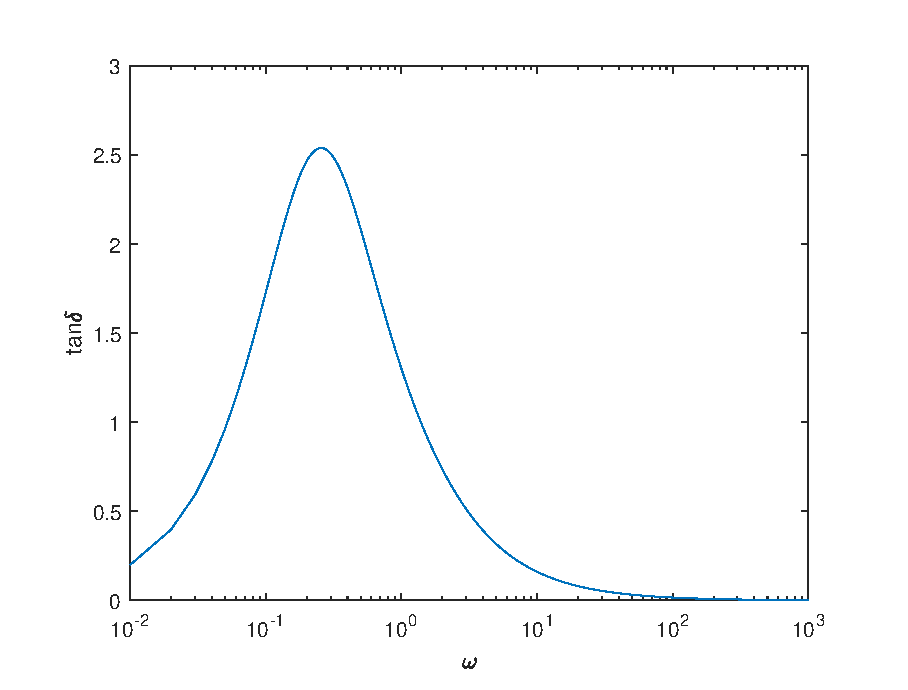
\includegraphics[width=0.7\linewidth]{hw-figures/HW3_P3b.eps}
    \caption{Tan($\delta$) vs $\omega$ plot}
    \label{fig:P3b}
\end{figure}
\newpage
\subsection*{3--4. \textbf{Fractional response} [4 pts].}

First following our generalized form for step strain:
\begin{equation}
    \sigma(t) = \int_{-\infty}^t G_r(t-\tau)\frac{d\varepsilon}{d\tau}d \tau
\end{equation}
we have
\begin{equation*}
    G_r(t) = \left[10 + 2\left(\frac{t}{0.2} \right)^{-\alpha}\right] \mathcal{H}(t),
\end{equation*}
and step strain:
\begin{equation}
    \varepsilon_0 \mathcal{H}(t)
\end{equation}
which gives us:
\begin{equation}
    \sigma(t) = \int_{-\infty}^t\left[10 + 2\left(\frac{t-\tau}{0.2} \right)^{-\alpha}\right] \mathcal{H}(t-\tau)\varepsilon_0 \delta (t) d \tau
\end{equation}
Now, plotting for each distinct alpha over a time range:
\begin{figure}[H]
    \centering
    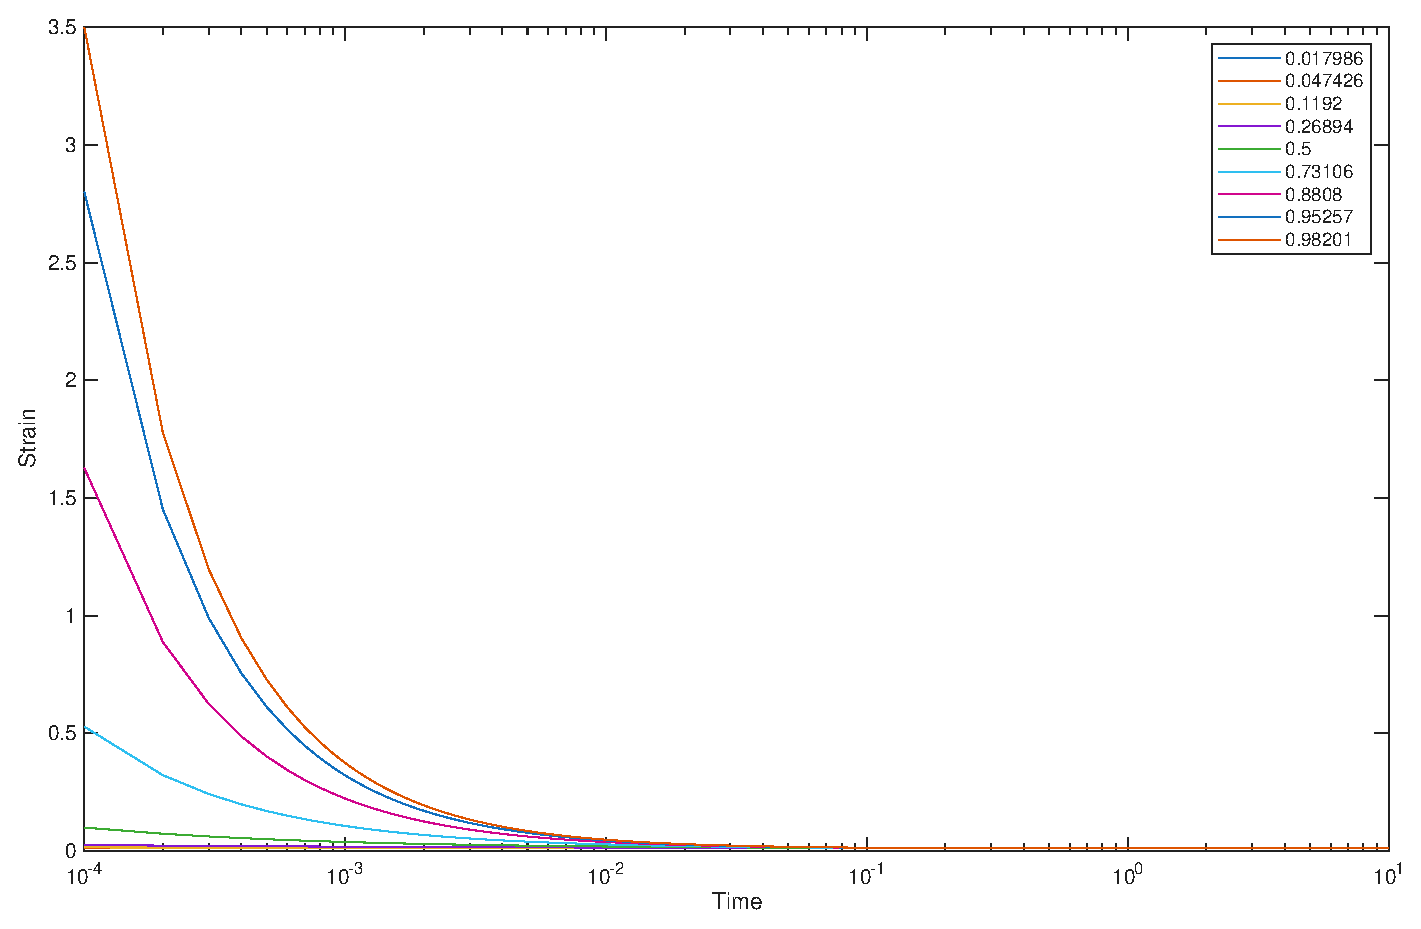
\includegraphics[width=0.7\linewidth]{hw-figures/HW3_P4a.eps}
    \caption{Strain vs Time plot}
    \label{fig:P4a}
\end{figure}
next for the step stress of length t=5:
\begin{equation}
    \varepsilon(t) = \int_{-\infty}^tJ_c(t-\tau) \frac{d\sigma}{d\tau}d\tau
\end{equation}
with out step stress defined by multiple heaviside functions:
\begin{equation}
    \sigma_0(\mathcal{H}(t)-\mathcal{H}(t-5)) 
\end{equation}
and Jc defined by:
\begin{equation}
    J_c = \mathcal{L}^{-1}(s^2*\mathcal{L}(G_r) )
\end{equation}
This operation did not work analytically so here is just the plot. I had to calculate the inverse laplace transform numerically in matlab for each alpha:
\begin{figure}[H]
    \centering
    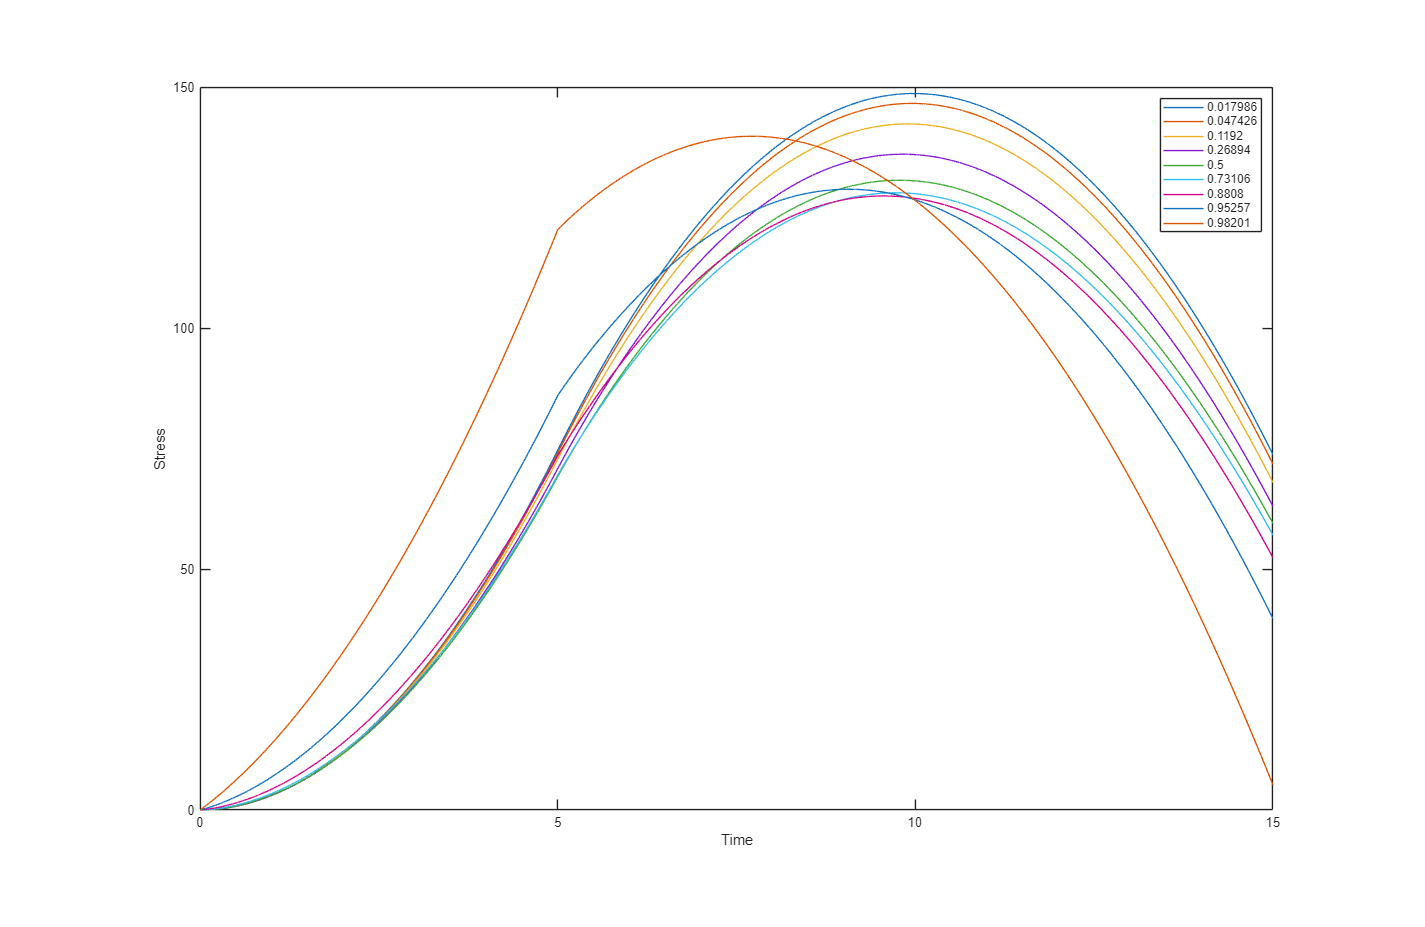
\includegraphics[width=0.7\linewidth]{hw-figures/HW3_P4b.eps}
    \caption{Stress vs Time plot}
    \label{fig:P4b}
\end{figure}
Now, for the final part, I have selected a cyclical step strain defined by the following combination of 
\begin{equation}
    \epsilon_0 (\mathcal{H}(t)-\mathcal{H}(t-5)+\mathcal{H}(t-10)-\mathcal{H}(t-15))
\end{equation}
which using out generalized form:
\begin{equation}
    \sigma(t) = \int_{-\infty}^t G_r(t-\tau)\frac{d\varepsilon}{d\tau}d \tau
\end{equation}
gives us:
\begin{equation}
    \sigma(t) = \int_{-\infty}^t \left[10 + 2\left(\frac{t-\tau}{0.2} \right)^{-\alpha}\right] \mathcal{H}(t-\tau)\varepsilon_0(\delta(\tau)-\delta(\tau-5)+\delta(\tau-10)-\delta(\tau-15))d \tau
\end{equation}
solving in mathematica and plotting for our various alphas and a time range of 20 seconds
\begin{figure}[H]
    \centering
    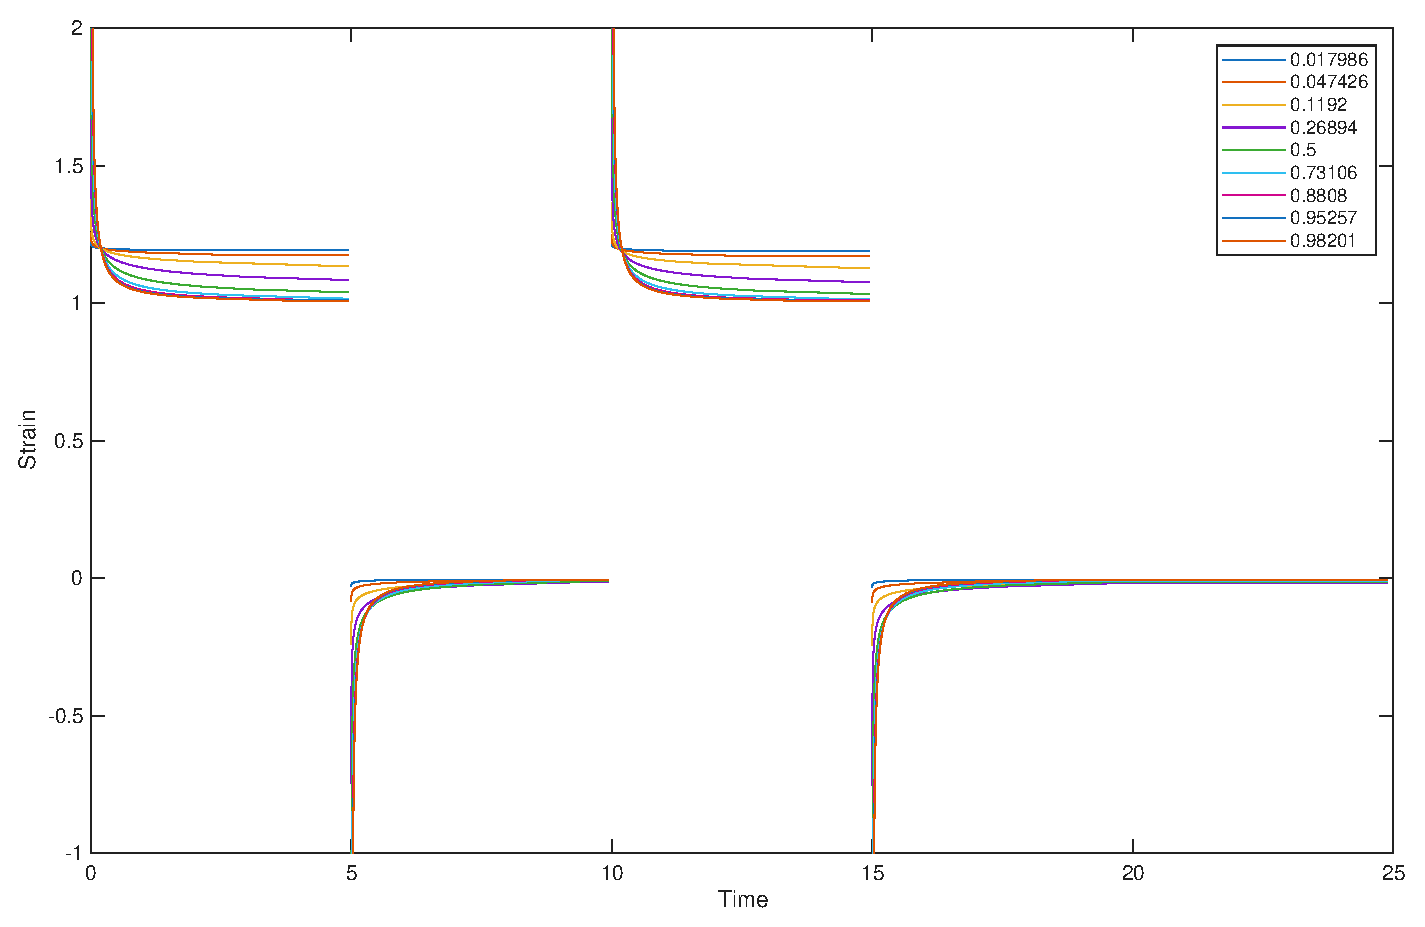
\includegraphics[width=0.7\linewidth]{hw-figures/HW3_P4c.eps}
    \caption{Strain vs Time plot}
    \label{fig:P4c}
\end{figure}

\bigskip
\bigskip
\subsection*{3--5. \textbf{Rheology without a rheometer} [8 pts].}
First, we can find the amount of energy from our initial height and rebound height:
\begin{equation}
    W_{diss} = mgh_0 - mgh(R)
\end{equation}
where:
\begin{equation}
    W_{diss} = 4/3\pi R^3\rho gh_0-  4/3\pi R^3 \rho gh(R)
\end{equation}
energy per volume:
\begin{equation}
     \boxed{W_{diss}/V =\rho gh_0-  \rho gh(R)}
\end{equation}

Now, to find the energy dissapated according to the lissajous plot, we start with strain energy:
\begin{equation}
    W_{store} = \frac{1}{2}\sigma\varepsilon
\end{equation}
knowing that the maximum energy is stored when displacement is the largest:
\begin{equation}
    W_{store} = \frac{1}{2}\sigma(\varepsilon_{max})\varepsilon_{max}
\end{equation}
looking at our Lissajous plot, we can see the triangle relating our maximum strain:
\begin{equation}
    \frac{\sigma(\varepsilon_{max})}{\varepsilon_{max}} = \cos(\delta)
\end{equation}
\begin{equation}
    \sigma(\varepsilon_{max}) = \varepsilon_{max}\cos(\delta)
\end{equation}
its worth noting that typically there would be an E' in there, but that is pulled out due to the $\sigma/|E^*|$ term. Plugging in:
\begin{equation}
    W_{store} = \frac{1}{2}\varepsilon_{max}^2\sin(\delta)
\end{equation}
now, since $\varepsilon_{max}$ is defined as B
\begin{equation}
    \boxed{W_{store} = \frac{1}{2}B^2\cos(\delta)}
\end{equation}

now, finding energy dissipated by ball drop event. Looking at the energy stored and dissipated equations we find:
\begin{equation}
    W_{diss} =\frac{1}{2}\sigma \varepsilon\frac{\pi}{2}\sin(\delta)
\end{equation}
once again defining our energy at the same point as the prior part, we can convert into terms of epsilon max:
\begin{equation}
    W_{diss} =\frac{\pi}{4} \varepsilon^2\sin(\delta)\cos(\delta)
\end{equation}
where, as before, note that our E' term vanished due to $\sigma/|E^*|$ . Now simplifying with the given terms:
\begin{equation}
    W_{diss} =\frac{\pi}{4} AB\cos(\delta)
\end{equation}
Now, to find tan delta as a function of rebound height:
\begin{equation}
    \Psi = 2\pi \tan(\delta)
\end{equation}
we can set equal to the energy dissipated from part a:
\begin{equation}
    4/3\pi R^3\rho gh_0-  4/3\pi R^3 \rho gh(R) =  2\pi \tan(\delta)
\end{equation}
dividing out:
\begin{equation}
    \boxed{\tan(\delta) = 2/3 R^3\rho g(h_0-  h(R))}
\end{equation}
now to find what frequencies this material is calibrated for, we can look at the hertzian contact relation and our tandelta versus R plot:

\begin{figure}[H]
    \centering
    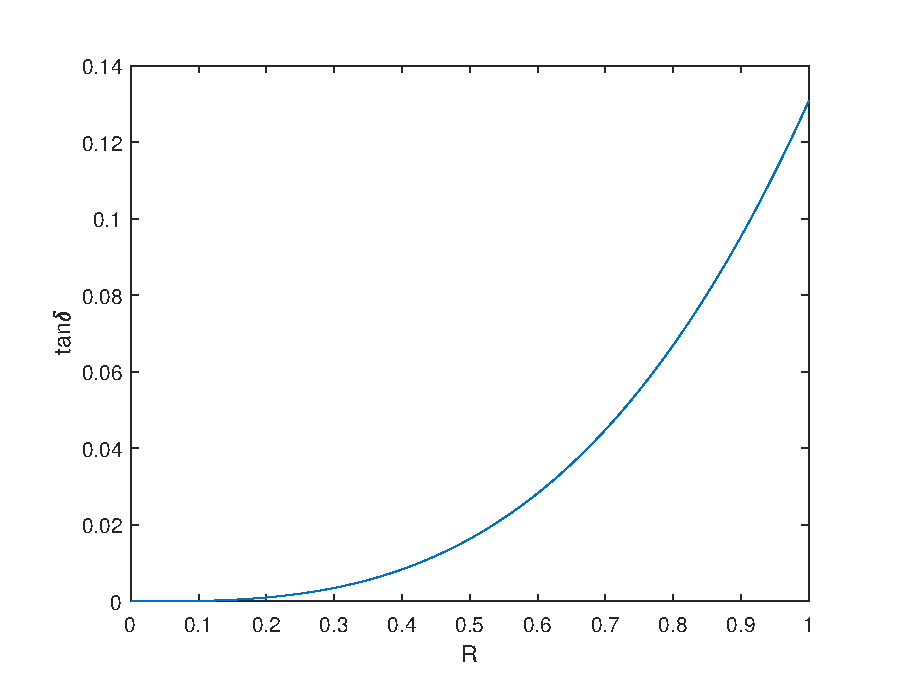
\includegraphics[width=0.7\linewidth]{hw-figures/HW3_P5e.eps}
    \caption{Tan($\delta$) vs R plot for h(R) = .08}
    \label{fig:P5e}
\end{figure}
from looking at this, which is over the given range of R, we see that the smallest tan deltas are for very small R values. in this case, lets pick .001m to .15 m for the range of R values this is calibrated. Now, from the contact relation we can find the time of impact, and then our frequency:
\begin{equation}
    t_{c,.001} = .025*.001 = .00025
\end{equation}
\begin{equation}
    t_{c,.15} = .025*.15 = .00375
\end{equation}
frequency..
\begin{equation}
    \omega = \frac{1}{t_c}
\end{equation}
Thus, our material is calibrated to lose the least energy between 266.67 Hz and 4000 Hz.
